\chapter{Threads}
\nt{
    Questo capitolo va studiato solo dopo il capitolo 9 sulla memoria centrale. Ai fini del programma del corso e dell’esame, si fa riferimento a queste slide, il cui contenuto è molto semplificato rispetto al capitolo 4 del libro di testo.
}

Consideriamo due processi che devono lavorare sugli stessi dati. Come possono farlo, se ogni processo ha la propria area dati (ossia, gli spazi di indirizzamento dei due processi sono separati)?

\begin{itemize}
    \item I due processi possono richiedere al sistema operativo un’area di memoria condivisa, oppure scambiarsi i dati usando messaggi.
    \item I dati possono essere mantenuti in un file, al quale i due processi accedono a turno.
\end{itemize}

Sarebbe comodo poter avere processi in grado di lavorare sugli stessi dati senza usare meccanismi espliciti di condivisione/comunicazione, e senza l’utilizzo di file, che risiedono su supporti relativamente lenti. Ad esempio, in un editor di testo:
\begin{itemize}
    \item Un processo gestisce l’input e i comandi di formattazione dell’utente;
    \item Un altro processo esegue il controllo automatico degli errori.
\end{itemize}

In questo caso, i due processi dovrebbero poter lavorare sullo stesso testo, la cui copia corrente è mantenuta in memoria principale. Tuttavia, poiché ogni processo ha un diverso spazio di indirizzamento, come possono lavorare sulla stessa copia dei dati?

Inoltre, durante il \textit{context switch} tra processi, occorre disattivare le aree dati e di codice del processo uscente e attivare quelle del processo entrante. 

\begin{itemize}
    \item Le \textbf{cache fisiche della CPU} contengono ancora i dati del processo uscente, quindi il processo entrante inizialmente genera molti \textit{miss cache}.
    \item Se due (o più) processi potessero condividere dati e codice, il context switch tra di loro sarebbe molto meno oneroso.
\end{itemize}

Da queste considerazioni nasce il concetto di \textbf{thread}: un gruppo di \textit{peer thread} è un insieme di “processi” che condividono lo spazio di indirizzamento (codice e dati).

\dfn{Terminologia}{
    Un processo $P$ (per come è stato studiato finora) è caratterizzato da un unico \textbf{Thread} di computazione: una sequenza di istruzioni eseguite, che ovviamente può cambiare da un’esecuzione all’altra in base, ad esempio, ai dati di input. (Fig. 4.1a).
}

Nessun altro processo ha accesso allo spazio di indirizzamento logico di $P$, quindi nessun processo utente, oltre a $P$, può accedere alle aree dati di $P$. Altri processi possono eseguire lo stesso codice di $P$, ma in uno spazio di indirizzamento logico separato e quindi con dati diversi. (Fig. 4.1a).

\section{Processo Multi-Thread}
Un \textbf{processo Multi-Thread} (o \textbf{Multi-Threaded}) è invece composto da più thread di computazione, detti \textit{peer thread}. Un processo multi-threaded è anche detto \textit{task} (Fig. 4.1).
\begin{figure}[h] \centering 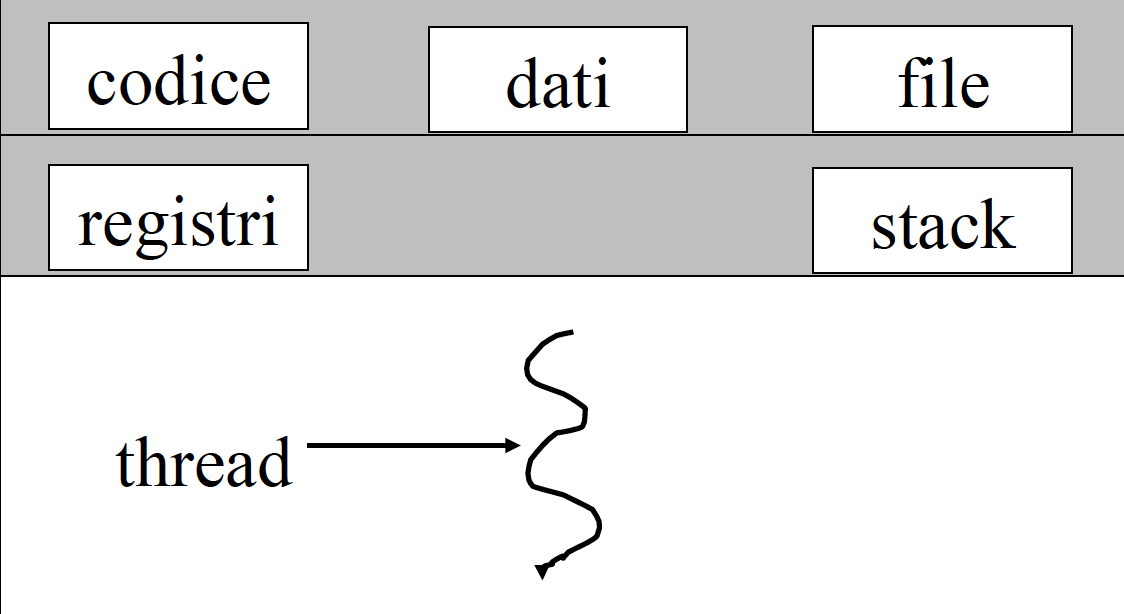
\includegraphics[width=0.50\linewidth]{images/thread_example.png} \caption{thread_example} \label{fig:4.1a} \end{figure}

\begin{figure}[h] \centering 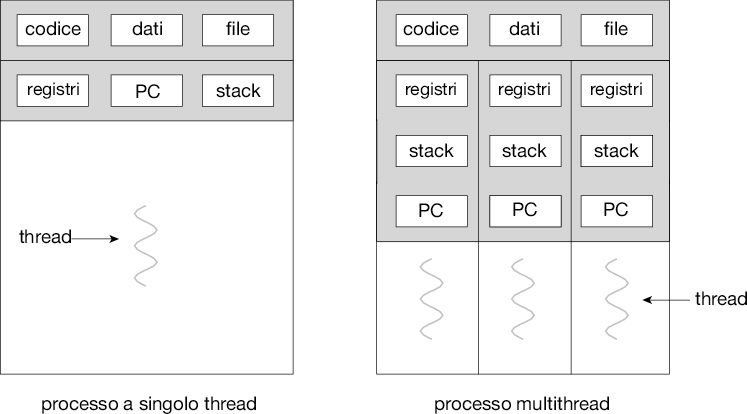
\includegraphics[width=0.50\linewidth]{images/MultiThreadExample.png} \caption{MultiThreadExample.png} \label{fig:4.2} \end{figure}
\dfn{Processo Multi-Thread}{
    Un processo \textbf{Multi-Thread} (o \textbf{Multi-Threaded}) è composto da più thread di computazione, detti \textit{peer thread}. Un processo multi-threaded è anche detto \textit{task} (Fig. 4.1).
}

Ad ogni \textit{peer thread} viene assegnata l’esecuzione di codice, che solitamente è diverso da quello degli altri peer thread. Di conseguenza:

\begin{itemize}
    \item Ogni thread ha uno stato di computazione autonomo, costituito da:
        \begin{itemize}
            \item \textbf{Program Counter} e registri della CPU
            \item uno \textbf{stack} indipendente
        \end{itemize}
    \item Tuttavia, un insieme di \textit{peer thread} condivide il codice in esecuzione e, soprattutto, le \textbf{aree dati}.
\end{itemize}

Il codice deve specificare quale \textit{peer thread} esegue ciascuna parte del codice, similmente a come, in un programma che utilizza la \texttt{fork}, si può definire la porzione di codice eseguita dal processo padre e quella eseguita dal processo figlio.

\clm{}{Context Switch tra Peer Thread}{
    Il \textit{context switch} avviene anche tra ciascun \textit{peer thread} di un processo multi-threaded, per permettere a ciascuno di continuare l’esecuzione del proprio codice assegnato. (Per ora si considera un’architettura \textbf{single core}.)
    
    \begin{itemize}
        \item Il \textit{context switch} tra \textit{peer thread} richiede solo il salvataggio e il ripristino del Program Counter, dei registri della CPU e dello stack, che sono distinti per ogni thread.
        \item Il codice e i dati, cioè lo \textbf{spazio di indirizzamento logico}, rimangono invariati tra \textit{peer thread}, per cui non è necessario cambiare la tabella delle pagine del processo multi-threaded durante il \textit{context switch}.
    \end{itemize}
}

Il \textit{context switch} tra processi è molto più oneroso per il SO rispetto a quello tra peer thread, poiché nel primo caso devono essere cambiate molte più informazioni.

\begin{itemize}
    \item A causa della gestione delle cache, il \textit{context switch} tra processi genera inizialmente più \textit{cache miss} rispetto a quello tra peer thread.
    \item Per questa ragione, i processi normali (quelli studiati finora) sono spesso chiamati \textbf{heavy-weight process} (HWP), mentre i \textit{peer thread} sono definiti \textbf{light-weight process} (LWP).
\end{itemize}

All'interno di un \textit{task}, nuovi peer thread possono essere creati tramite apposite \textit{system call}, e a ciascun thread può essere assegnato codice specifico da eseguire, in modo simile a quanto avviene con \texttt{fork} ed \texttt{exec}. (In \textbf{Linux} un nuovo thread si crea con la system call \texttt{clone}, mentre in \textbf{Windows} con \texttt{CreateThread}.)

\nt{
    Altre \textit{system call} permettono ai peer thread di sincronizzarsi fra loro, analogamente a come i processi possono sincronizzarsi tramite semafori. La sincronizzazione è fondamentale per garantire un accesso ordinato ai dati condivisi tra i thread. Inoltre, molti linguaggi moderni, come Java, offrono primitive apposite per la programmazione multi-threaded.
}

In tutti i sistemi operativi moderni, la gestione dello \textbf{scheduling} dei thread avviene a livello di \textit{kernel}. Il SO mantiene strutture dati per gestire sia i processi normali che tutti i peer thread di un \textit{task} multi-threaded.

\begin{itemize}
    \item Quando un thread si blocca volontariamente o termina il suo quanto di tempo, è il SO a gestire l'assegnazione della CPU, decidendo se assegnarla:
        \begin{itemize}
            \item ad un altro \textit{peer-thread} dello stesso task,
            \item ad uno dei \textit{peer-thread} di un altro task,
            \item oppure ad un processo normale.
        \end{itemize}
\end{itemize}
\nt{
    In Solaris, la creazione di un nuovo \textbf{LWP} (light-weight process) richiede circa 30 volte meno tempo rispetto alla creazione di un \textbf{HWP} (heavy-weight process). Inoltre, il \textit{context switch} tra peer thread è cinque volte più rapido rispetto al \textit{context switch} tra processi.
}

\begin{itemize}
    \item \textbf{Condivisione di dati e risorse}: più thread possono accedere e operare su dati condivisi in modo efficiente, anche se devono essere sincronizzati adeguatamente per evitare condizioni di gara o accessi non sicuri ai dati.
    \item \textbf{Architetture multi-core}: i thread sono particolarmente idonei per essere eseguiti su processori multi-core e, ancor di più, su architetture multithreaded.
\end{itemize}

In un processore \textit{single-core}, tutti i \textit{peer thread} di un task si alternano in esecuzione esattamente come un insieme di processi (Figura 4.3). Come già osservato, il \textit{context switch} tra vari \textit{peer thread} è meno oneroso rispetto al \textit{context switch} tra processi normali. Tuttavia, un \textit{context switch} con un altro processo rimane oneroso e può causare un degrado nelle prestazioni a causa dei miss di cache generati inizialmente dal processo entrante.

\begin{itemize}
    \item \textbf{Architetture multi-core e task multi-threaded}: le architetture multi-core sono particolarmente adatte alla gestione di task multi-threaded. Supponiamo un sistema \textbf{dual-core} in cui sono attivi due task multi-threaded: se si assegna un task a ciascun core, i \textit{context switch} tra thread saranno limitati ai soli \textit{peer thread} del medesimo task, ottimizzando l’efficienza.
    \item \textbf{Bilanciamento del carico}: in pratica, il numero totale di task multi-threaded (e quindi di \textit{peer thread}) è spesso superiore al numero di core disponibili. Il sistema operativo distribuisce quindi i \textit{peer thread} di uno stesso task su core diversi per bilanciare il carico di lavoro in modo ottimale (Figura 4.4 mostra un task con 4 \textit{peer thread} distribuito su due core).
\end{itemize}

\cor{Opportunità di esecuzione parallela nei processori moderni}{
    I processori moderni offrono un'opportunità ulteriore per l'esecuzione dei thread. In un processore multicore, ciascun core è in grado di eseguire fino a 4 o 5 istruzioni in parallelo del programma in esecuzione; questa tecnica è nota come \textbf{multiple issue}.
    
    \begin{itemize}
        \item Per eseguire più istruzioni in parallelo, ogni core deve disporre di più unità funzionali, come le ALU (Arithmetic Logic Units) e le unità di calcolo in virgola mobile. Tale struttura è detta \textit{superscalare}, poiché consente a ciascun core di eseguire in parallelo fino a 4 o 5 istruzioni, migliorando l'efficienza complessiva del sistema.
    \end{itemize}
}
